% Number 310
% CVPMG  Units
% Graph description, problem-solving
% JG

% Watermark
\AddToShipoutPicture*{\BackgroundPic}

\addtocounter {ProbNum} {1}

%\begin{floatingfigure}[r]{.3\textwidth}
%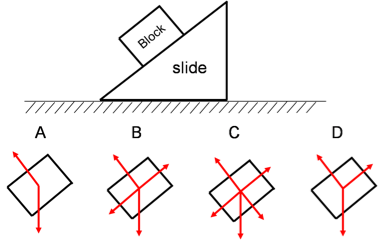
\includegraphics[scale=.4]{/Users/jgates/desktop/latex/pics/incline3.png}
%\end{floatingfigure}
 
{\bf \Large{\arabic{ProbNum}}}An exciting chase has broken out between a toy police car and a toy speeder (running from the police because he foolishly doesn�t have any toy insurance).  
 
\begin{center}
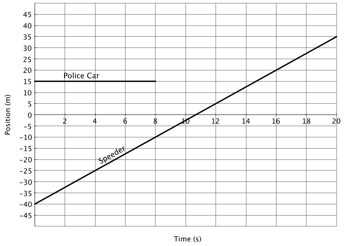
\includegraphics[scale=.87]{/Users/jgates/desktop/latex/pics/cvpm2.png}
\end{center}

\bigskip
Describe the segment of the chase shown so far, as accurately as you can (ie: including exact values).
 
\vspace{40mm}
Assuming that the toy police car can get up to speed very quickly, how fast will it need to go in order to catch the speeder before ${t=~}$20 s?

\vfill

\newpage